\section{VLAN}
\label{sec:vlan}
Virtuální LAN slouží k \textbf{logického rozdělení sítě nezávisle na fyzickém uspořádání}.
Lze tímto síť LAN segmentovat na menší sítě uvnitř \textbf{jedné fyzické struktury}.
Touto technologií dosáhneme výsledků, jako bychom tyto sítě měli připojené do samostného switche, ale na switchi jednom. \\
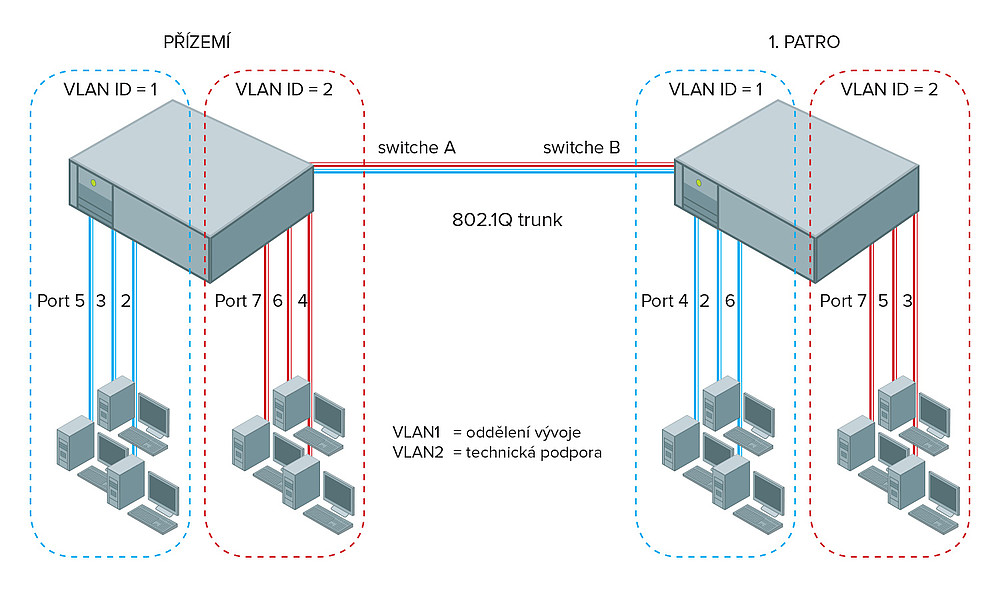
\includegraphics[width=\linewidth]{TVY-POS/VLAN/VLAN.jpg}

Tyto sítě jsou na sobě \textbf{nezávislé, nemohou spolu komunikovat}.
K zajištění komunikace mezi sítěmi \textbf{je nutno použít směrování}.
V dnešní době je možno využít \textbf{L3 switch či router}.

Jelikož komunikace po první a druhé vrstvě ISO/OSI toto rozdělení není možna zajístit, je nutné zařízením nastavit ignorování komunikace jiné sítě VLAN.
Komunikaci \textbf{je možné tímto způsobem odposlouchávat}.
Z tohoto důvodu se využívá L3 switchů a routerů schopných komunikaci \textbf{rozesílat pouze na požadované porty}. \\
\\
Důvody pro použití VLAN:
\begin{itemize}
  \item \textbf{Seskupování uživatelů} v síti podle skupin či oddělení nebo podle služeb místo podle fyzického umístění a oddělení komunikace mezi těmito skupinami
  \item \textbf{Snížení broadcast domén} v síti, které začaly být problémem již před několika lety
  \item \textbf{Zmenšení kolizních domén} v době, kdy se ještě používaly huby
\end{itemize}
Vhodné rozdělení uživatelů do VLAN:
\begin{itemize}
  \item \textbf{Podle organizační struktury} - pokud je většina komunikace v rámci oddělení, kde jsou vlastní tiskárny, file servery, \dots a mezi jednotlivými odděleními není komunikace, pouze pár služeb (mail) je společných pro všechny
  \item \textbf{Podle služeb} - do VLAN se seskupují pracovníci, kteří využívají stejné služby (Účetnictví, DB, \dots)
\end{itemize}
Výhody VLAN:
\begin{itemize}
  \item \textbf{Snížení broadcastů} - Vyšší výkon sítě
  \item \textbf{Zjednodušení správa} - K přesunu zařízení mezi VLAN je možné využít SW konfiguraci, není nutné šahat na HW
  \item \textbf{Zvýšení zabezpečení} - Oddělení komunikace, ke které poté není přístup
  \item \textbf{Oddělení speciálního provozu} - Neovlivňuje běžný provoz
  \item \textbf{Cena} (HW náročnost) - Možné využití jednoho switche pro více VLAN
\end{itemize}
\subsection{Způsoby zařezení zařízení do VLAN}
\begin{enumerate}
  \item \textbf{Podle portu} switche/routeru - Port switche má pevně stanoven jaký port přísluší jaké VLAN.
        Nejrychlejší a nejpoužívanější řešení.
  \item \textbf{Podle MAC adresy} zařízení - Switch hledá v databázi MAC adresu připojeného zařízení, podle které určuje do jaké VLAN zařízení připojí.
        Velmi náročné na výkon a administraci.
  \item \textbf{Podle protokolu} (Informací z 3. vrstvy) - Oddělení provozu podle IP adres či typu komunikace (AppleTalk)
        V praxi není příliš rozšířené.
  \item \textbf{Podle autentizace} - Zařízení se autentizuje pomocí RADIUS serveru a podle údajů se přiřadí do VLAN.
        Velmi univerzální.
\end{enumerate}
\subsection{Komunikace v rámci VLAN}
\subsubsection{Pomocí jednoho switche}
Switch si v operační paměti udržuje informace, do které VLAN patří daná komunikace a v rámci switche povoluje pouze správné směrování.
V tomto případě jsou jednotlivé porty switche buďto staticky nebo dynamicky (Podle způsobu zařazení zařízení do VLAN) zařazeny do jednotlivé VLAN.
\subsubsection{Pomocí více switchů}
Jestliže požadujeme, aby se informace o zařazení do VLAN mezi switchi neztratila, je nutné využít nějakou metodu zajišťující správný průběh.
Pokud se využívá rozdělení pomocí MAC adres zařízení, je nutné, aby si switche mezi sebou sdílely databázy MAC adres.
Firma Cisco si vytvořila vlastní metodu zvanou ISL, která přenásí informace potřebné ke správnému přenosu v rámcích komunikace, funguje ovšem pouze na zařízeních Cisco.

Nejvíce se v dnešní době používá standard IEEE 802.1Q, který značkuje rámce komunikace pouze v případě, že komunikace probíhá v rámci více switchů.
Tento standard do rámce přidává informaci o zařazení zařízení do VLAN na portu switche a na druhé straně se tato informace rozbalí a rámec se pošle správnému zařízení.
Port na kterém dochází k odchozí komunikaci do jiného switche se nazývá \textbf{trunk} port.
Spoj mezi dvěma trunk porty se nazývá \textbf{trunk} nebo \textbf{trunk link}.
\subsubsection{Native VLAN}
Na trunk portu je možné nastavit tzv. "Native VLAN", na kterém nedochází k značkování ramců komunikace.
Jestliže se na trunk port dostane rámec, který nemá tag, tak je automaticky přiřazen Native VLAN.
\subsection{Komunikace mezi VLAN}
K VLAN se můžeme chovat jako k podsítím, tudíž je možné komunikaci provádět pomocí routeru a switche, který každou podsíť připojí samostatným kabelem, nebo jedním v konfiguraci router-on-a-stick. \\
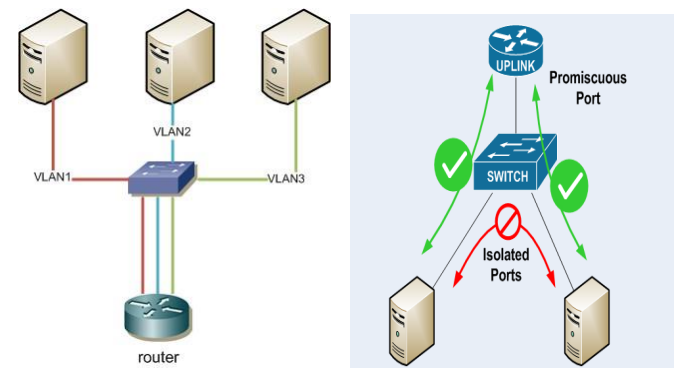
\includegraphics[width=\linewidth, height=6cm]{TVY-POS/VLAN/VLAN-router.png}
Mnohem lepší a výhodnější je ovšem využít zmiňovaných trunků a případně L3 switche, který je rychlejší.
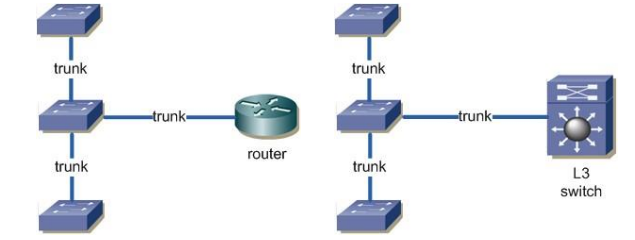
\includegraphics[width=\linewidth]{TVY-POS/VLAN/VLAN-trunk.png}
